% !TeX spellcheck = en_GB 

\section{\label{sec::modelling}Modelling the cake}
To model the baking process, we now only need a few more ingredients. First we have to know the thermal properties of cake dough and the baking form, which we will consider to be out of aluminium. For the dough \cite{baik1999modeling} found out, that the thermal diffusivity of cupcake dough, which should be close enough to our cake dough is $\alpha_{cake} =  1.02\times 10^{-7} \SI{}{\meter/\second^2} - 1.698\times 10^{-7} \SI{}{\meter/\second^2}$. For the thermal diffusivity of aluminium the appendix of \cite{kothandaraman2006fundamentals} gives us $\alpha_{Al} = 9.444\times 10^{-5} \SI{}{\meter/\second^2}$.

Second we need the mesh, which models. This was given by the task and can be seen in figure \ref{fig::mesh}, where the yellow part identifies an aluminium stick, which will help to heat up the cake from the inside. For the radius we chose $15\SI{}{\centi\meter}$, as we wanted to have a big cake, which had a realistic chance, to get baked in a reasonable time.

\begin{figure}[htp]
	\centering
	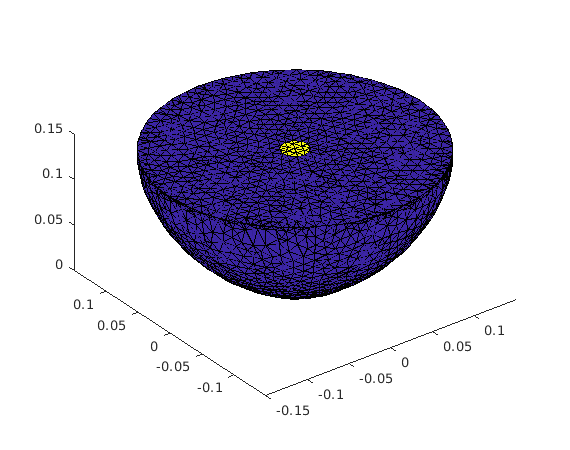
\includegraphics[width=0.5\textwidth]{figures/mesh.png}
	\caption{\label{fig::mesh} Mesh of the cake}
\end{figure}